% ============================================================
% Figure 3: Scene Graph Constraint Reasoning Visualization
% Shows scene graph construction and constraint inference
% Compile: pdflatex fig_scene_graph.tex
% ============================================================
\documentclass[border=3pt]{standalone}
\usepackage{tikz}
\usetikzlibrary{
  positioning, arrows.meta, shapes.geometric, fit, backgrounds,
  calc, decorations.pathreplacing, shadows.blur
}
\usepackage{xcolor}
\usepackage{times}
\usepackage{amsmath}

% Colors
\definecolor{objblue}{HTML}{2E86C1}
\definecolor{objgreen}{HTML}{27AE60}
\definecolor{objred}{HTML}{E74C3C}
\definecolor{objorange}{HTML}{E67E22}
\definecolor{edgegray}{HTML}{7F8C8D}
\definecolor{constpurple}{HTML}{8E44AD}
\definecolor{adjustteal}{HTML}{17A589}
\definecolor{bglight}{HTML}{F8F9FA}
\definecolor{fragilered}{HTML}{CB4335}

\begin{document}
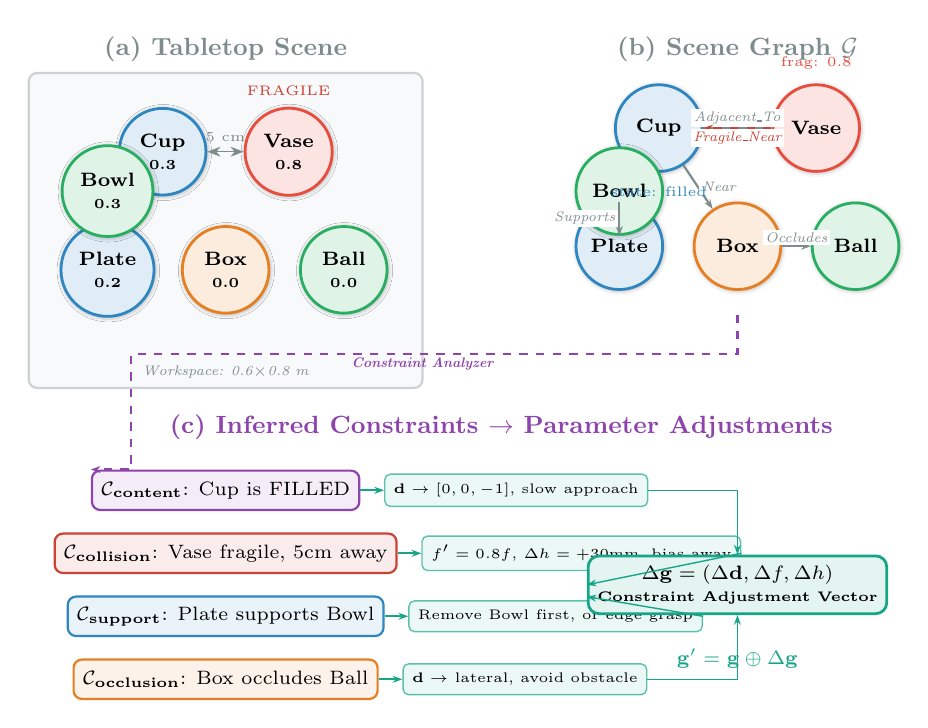
\begin{tikzpicture}[
  >=Stealth,
  node distance=0.5cm,
  objnode/.style={
    circle, draw=#1, fill=#1!15, line width=1pt,
    minimum size=1.1cm, font=\scriptsize\bfseries, text=black, align=center,
    blur shadow={shadow blur steps=3, shadow xshift=0.3pt, shadow yshift=-0.3pt}
  },
  edgelabel/.style={
    font=\tiny\itshape, text=edgegray, fill=white, inner sep=1pt
  },
  constbox/.style={
    rectangle, rounded corners=3pt,
    draw=#1, fill=#1!10, line width=0.8pt,
    minimum width=3cm, minimum height=0.5cm,
    font=\scriptsize, text=black, align=left
  },
  adjustbox/.style={
    rectangle, rounded corners=2pt,
    draw=adjustteal!70, fill=adjustteal!8, line width=0.5pt,
    font=\tiny, text=black, align=left
  },
  myarrow/.style={
    ->, line width=0.8pt, color=#1,
    >={Stealth[length=3.5pt, width=2.5pt]}
  },
  groupbox/.style 2 args={
    rectangle, rounded corners=6pt,
    draw=#1, fill=#2, line width=1.2pt, inner sep=8pt
  }
]

% ================================================================
% LEFT: Scene Layout (top-down view of tabletop)
% ================================================================
\node[font=\small\bfseries, text=edgegray] at (0, 4.8) {(a) Tabletop Scene};

% Table surface
\draw[fill=bglight, draw=edgegray!40, rounded corners=3pt, line width=0.8pt]
  (-2.5, 0.5) rectangle (2.5, 4.5);
\node[font=\tiny\itshape, text=edgegray] at (0, 0.7) {Workspace: 0.6$\times$0.8 m};

% Objects on table
\node[objnode=objblue] (cup) at (-0.8, 3.5) {Cup\\{\tiny 0.3}};
\node[objnode=objred] (vase) at (0.8, 3.5) {Vase\\{\tiny 0.8}};
\node[objnode=objgreen] (ball) at (1.5, 2) {Ball\\{\tiny 0.0}};
\node[objnode=objorange] (box) at (0, 2) {Box\\{\tiny 0.0}};
\node[objnode=objblue] (plate) at (-1.5, 2) {Plate\\{\tiny 0.2}};
\node[objnode=objgreen] (bowl) at (-1.5, 3) {Bowl\\{\tiny 0.3}};

% Fragility labels
\node[font=\tiny, text=fragilered] at ($(vase.north)+(0,0.2)$) {FRAGILE};

% Distance annotation
\draw[<->, line width=0.4pt, edgegray] (cup.east) -- (vase.west)
  node[midway, above, font=\tiny, text=edgegray] {5 cm};

% ================================================================
% CENTER: Scene Graph
% ================================================================
\node[font=\small\bfseries, text=edgegray] at (6.5, 4.8) {(b) Scene Graph $\mathcal{G}$};

% Graph nodes
\node[objnode=objblue] (gcup) at (5.5, 3.8) {Cup};
\node[objnode=objred] (gvase) at (7.5, 3.8) {Vase};
\node[objnode=objgreen] (gball) at (8, 2.3) {Ball};
\node[objnode=objorange] (gbox) at (6.5, 2.3) {Box};
\node[objnode=objblue] (gplate) at (5, 2.3) {Plate};
\node[objnode=objgreen] (gbowl) at (5, 3) {Bowl};

% Graph edges with labels
\draw[myarrow=edgegray] (gcup) -- (gvase)
  node[edgelabel, midway, above] {Adjacent\_To};
\draw[myarrow=edgegray] (gbox) -- (gball)
  node[edgelabel, midway, above] {Occludes};
\draw[myarrow=edgegray] (gplate) -- (gbowl)
  node[edgelabel, midway, left] {Supports};
\draw[myarrow=edgegray] (gcup) -- (gbox)
  node[edgelabel, midway, right] {Near};
\draw[myarrow=fragilered, dashed, line width=0.6pt] (gvase) -- (gcup)
  node[edgelabel, midway, below, text=fragilered] {Fragile\_Near};

% Node attribute annotations
\node[font=\tiny, text=objblue, below=0.05cm of gcup] {state: filled};
\node[font=\tiny, text=objred, above=0.05cm of gvase] {frag: 0.8};

% ================================================================
% BOTTOM: Constraint Inference
% ================================================================
\node[font=\small\bfseries, text=constpurple] at (3.5, 0) {(c) Inferred Constraints $\to$ Parameter Adjustments};

% Constraint types with adjustments
\node[constbox=constpurple] (c1) at (0, -0.8) 
  {\textbf{$\mathcal{C}_{\text{content}}$}: Cup is FILLED};
\node[adjustbox, right=0.3cm of c1] (a1) 
  {$\mathbf{d} \to [0,0,{-}1]$, slow approach};

\node[constbox=fragilered] (c2) at (0, -1.6) 
  {\textbf{$\mathcal{C}_{\text{collision}}$}: Vase fragile, 5cm away};
\node[adjustbox, right=0.3cm of c2] (a2) 
  {$f' = 0.8f$, $\Delta h = {+}30$mm, bias away};

\node[constbox=objblue] (c3) at (0, -2.4) 
  {\textbf{$\mathcal{C}_{\text{support}}$}: Plate supports Bowl};
\node[adjustbox, right=0.3cm of c3] (a3) 
  {Remove Bowl first, or edge grasp};

\node[constbox=objorange] (c4) at (0, -3.2) 
  {\textbf{$\mathcal{C}_{\text{occlusion}}$}: Box occludes Ball};
\node[adjustbox, right=0.3cm of c4] (a4) 
  {$\mathbf{d} \to$ lateral, avoid obstacle};

% Arrows from constraints to adjustments
\draw[myarrow=adjustteal] (c1.east) -- (a1.west);
\draw[myarrow=adjustteal] (c2.east) -- (a2.west);
\draw[myarrow=adjustteal] (c3.east) -- (a3.west);
\draw[myarrow=adjustteal] (c4.east) -- (a4.west);

% Final output
\node[rectangle, rounded corners=4pt, draw=adjustteal, fill=adjustteal!12, 
  line width=1pt, font=\scriptsize\bfseries, text=black, align=center,
  minimum width=3.5cm, minimum height=0.6cm] (deltaG) at (6.5, -2) 
  {$\Delta\mathbf{g} = (\Delta\mathbf{d}, \Delta f, \Delta h)$\\
  {\tiny Constraint Adjustment Vector}};

% Arrows from adjustments to deltaG
\draw[myarrow=adjustteal, line width=0.5pt] (a1.east) -| (deltaG.north);
\draw[myarrow=adjustteal, line width=0.5pt] (a2.east) -- (deltaG.west);
\draw[myarrow=adjustteal, line width=0.5pt] (a3.east) -- ($(deltaG.west)+(0,-0.15)$);
\draw[myarrow=adjustteal, line width=0.5pt] (a4.east) -| (deltaG.south);

% Final formula
\node[font=\scriptsize\bfseries, text=adjustteal, below=0.3cm of deltaG] 
  {$\mathbf{g}' = \mathbf{g} \oplus \Delta\mathbf{g}$};

% Connection from scene graph to constraints
\draw[myarrow=constpurple, line width=0.8pt, dashed] ($(gbox.south)+(0, -0.3)$) -- ++(0, -0.5) -| 
  ($(c1.north)+(-1.2, 0.3)$) -- ($(c1.north)+(-1.2, 0)$) -- (c1.north west);
\node[font=\tiny\bfseries\itshape, text=constpurple] at (2.5, 0.8) {Constraint Analyzer};

\end{tikzpicture}
\end{document}
